\section*{Methodology}

\subsection*{PyKEEN}

PyKEEN~\cite{pykeen} is an open-source Python library that facilitates training and evaluation of knowledge graph embedding models.
It streamlines the process of embedding entities and relations into continuous vector spaces, enabling efficient link prediction and relationship classification.
PyKEEN supports a wide range of models, including TransE, RotatE, ComplEx, and DistMult, each with unique characteristics and performance profiles.

In this project, PyKEEN was used to predict missing links within a knowledge graph through a structured workflow involving data extraction, preparation, model training, and link prediction.

\subsection*{Knowledge Graph Embeddings for Link Prediction}

In our experiments, we focused on two primary approaches for knowledge graph completion: traditional knowledge graph embedding models and LLM-based embeddings (detail in Section Model Evaluation). Among knowledge graph embedding models available in PyKEEN, in this first iteration we used several families of models starting from the simplest approaches.
\begin{itemize}
    \item \textbf{Translational Models (Distance-based)}: TransE~\cite{10.5555/2999792.2999923}, TransH~\cite{10.5555/2893873.2894046}, TransR~\cite{10.5555/2886521.2886624}, and TransD~\cite{ji-etal-2015-knowledge}.
    This family of models embeds entities and relations in the same space, with the distance between head and tail entities reflecting the relationship.
    \item \textbf{Rotational Models}: RotatE~\cite{sun2019rotateknowledgegraphembedding} is a rotational model that represents relations as rotations in the complex vector space. This model has shown state-of-the-art performance on several benchmark datasets.
    \item \textbf{Semantic Matching Models (Tensor Factorization-based)}: DistMult~\cite{yang2015embeddingentitiesrelationslearning }, RESCAL~\cite{10.5555/3104482.3104584}, and TuckER~\cite{Balazevic_2019} are semantic matching models that capture complex interactions between entities and relations. These models are more expressive than translational models and have shown competitive performance on various datasets.
\end{itemize}

\subsection*{Neo4j Desktop}

Neo4j Desktop \cite{neo4j} serves as a crucial tool for managing and querying the knowledge graph used in this project.
It provides a local environment to import, visualize, and manipulate graph data, facilitating seamless interaction with datasets.
Central to this process is Neo4j's support for Cypher, a declarative graph query language that efficiently extracts triples representing relationships between entities.
These triples $(h, r, t)$---comprising head entities, relationships, and tail entities---form the backbone of the knowledge graph.

After retrieval through Cypher queries (Listing~\ref{lst:cypher_query}), the triples can then be converted into PyKEEN's \texttt{TriplesFactory} format, facilitating integration with the PyKEEN pipeline for link prediction and multi-class relationship classification.

\begin{lstlisting}[caption=Cypher query to retrieve triples., label=lst:cypher_query]
    MATCH (h)-[r]->(t)
    RETURN id(h) AS head, type(r) AS relation, id(t) AS tail
\end{lstlisting}

\subsubsection*{Setup and Database Import}

This section provides a step-by-step guide to set up Neo4j Desktop and import a database dump file, as depicted in Figure~\ref{fig:neo4j-setup}. The specific dump used in this midterm report, derived from Hetionet, requires DBMS version $4.3$ to ensure compatibility.

\begin{figure}
    \centering
    \begin{subfigure}[b]{0.49\textwidth}
        \centering
        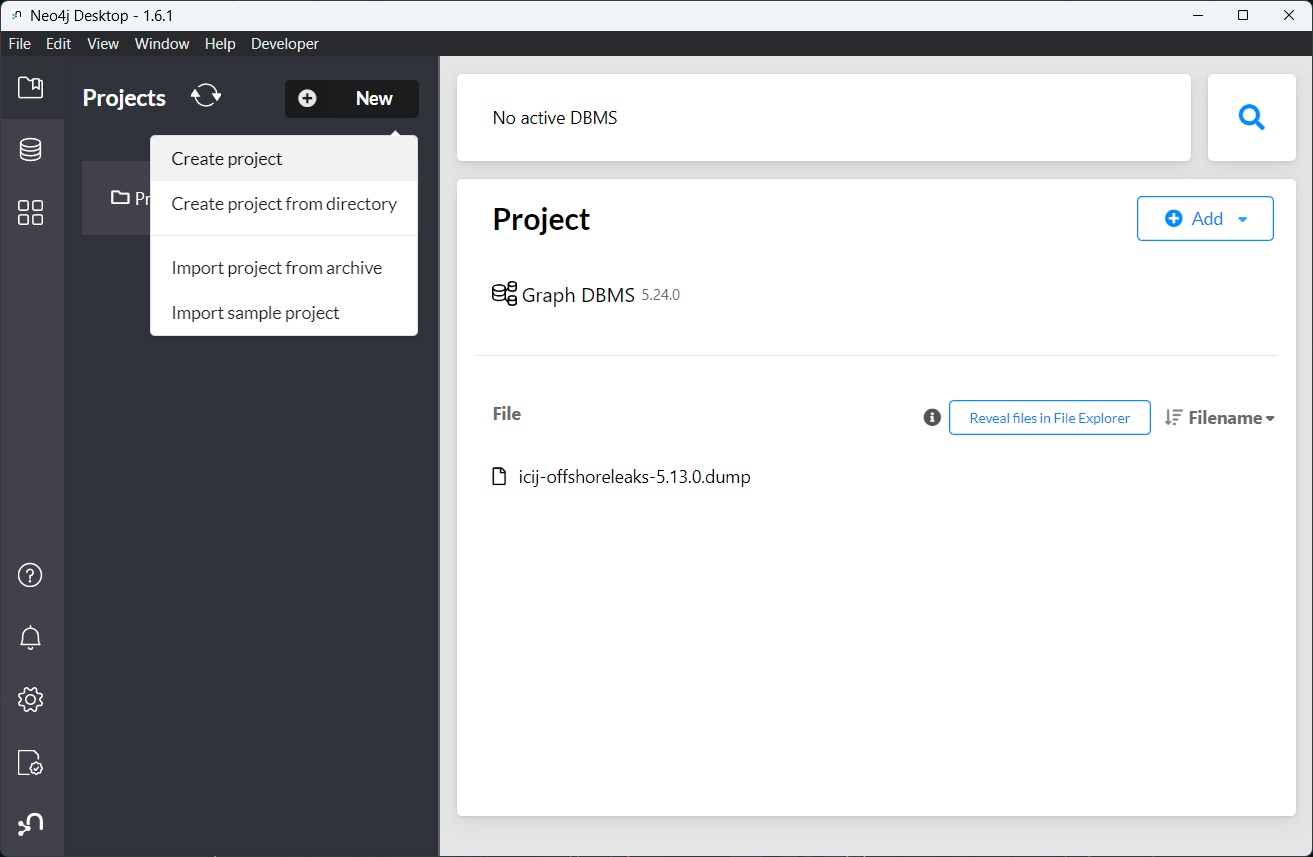
\includegraphics[width=\textwidth]{images/neo4j-setup/1}
        \caption{Creating a project.}
    \end{subfigure}
    \hfill
    \begin{subfigure}[b]{0.49\textwidth}
        \centering
        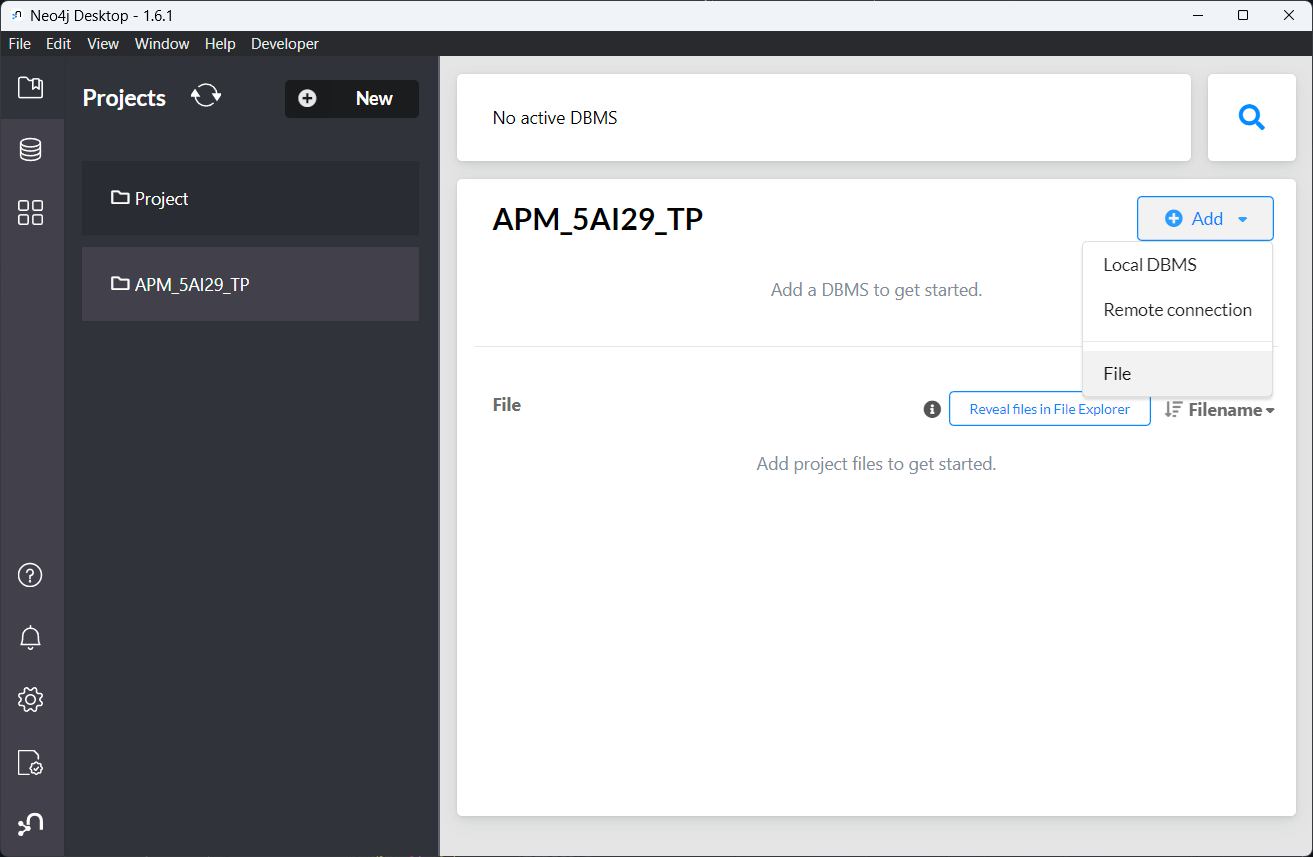
\includegraphics[width=\textwidth]{images/neo4j-setup/2}
        \caption{Adding dump file.}
    \end{subfigure}
    \\
    \begin{subfigure}[b]{0.49\textwidth}
        \centering
        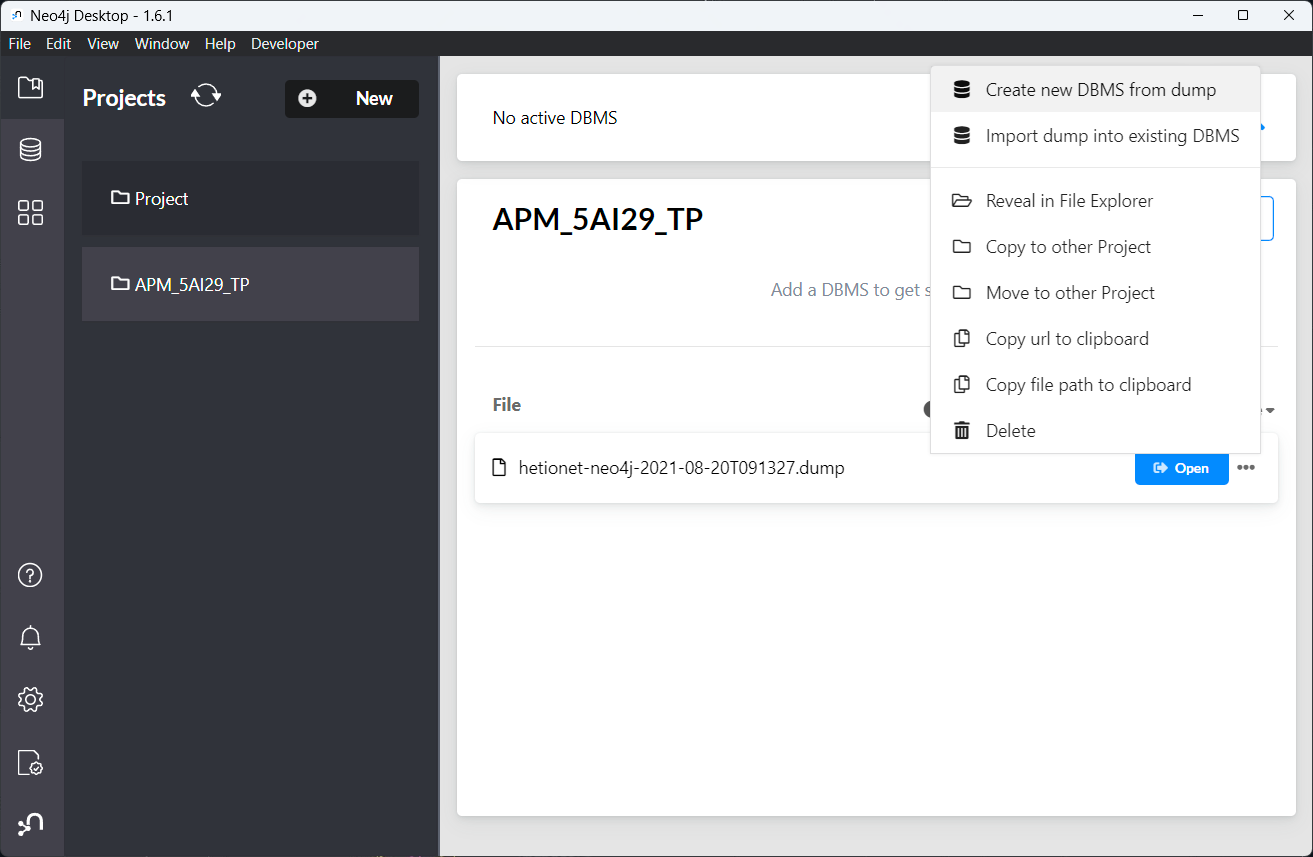
\includegraphics[width=\textwidth]{images/neo4j-setup/3}
        \caption{Importing dump to DBMS.}
    \end{subfigure}
    \hfill
    \begin{subfigure}[b]{0.49\textwidth}
        \centering
        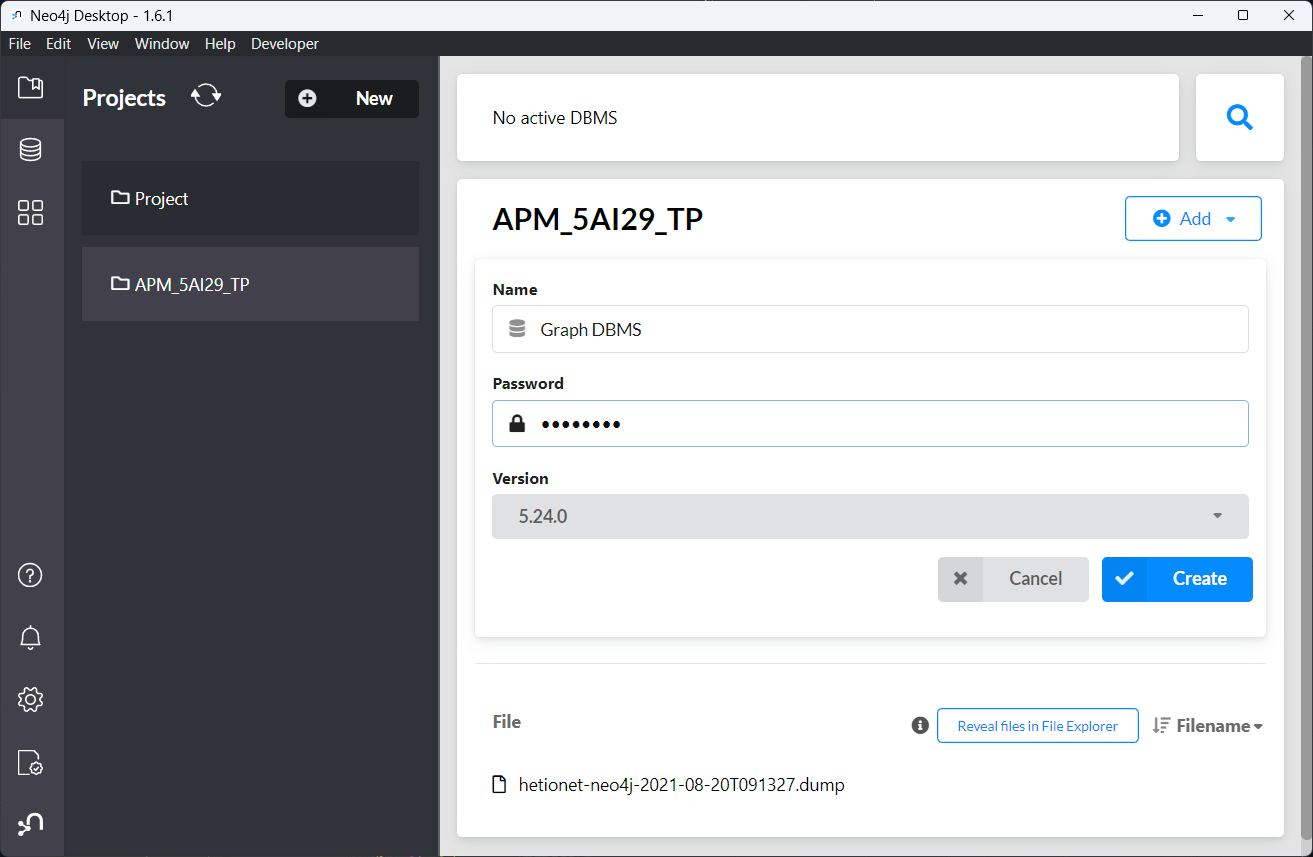
\includegraphics[width=\textwidth]{images/neo4j-setup/4}
        \caption{Configuring DBMS.}
    \end{subfigure}
    \\
    \begin{subfigure}[b]{0.49\textwidth}
        \centering
        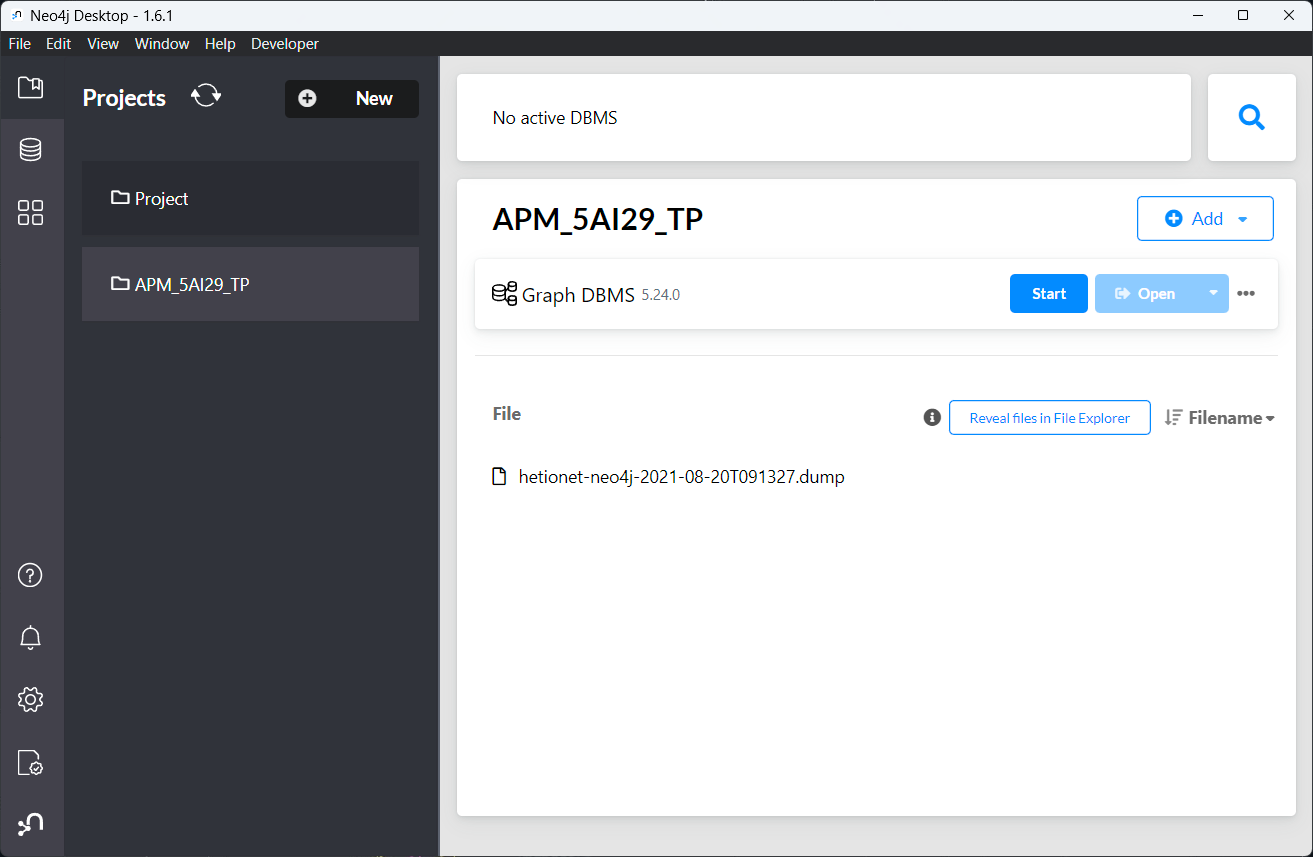
\includegraphics[width=\textwidth]{images/neo4j-setup/5}
        \caption{Starting DBMS.}
    \end{subfigure}
    \hfill
    \begin{subfigure}[b]{0.49\textwidth}
        \centering
        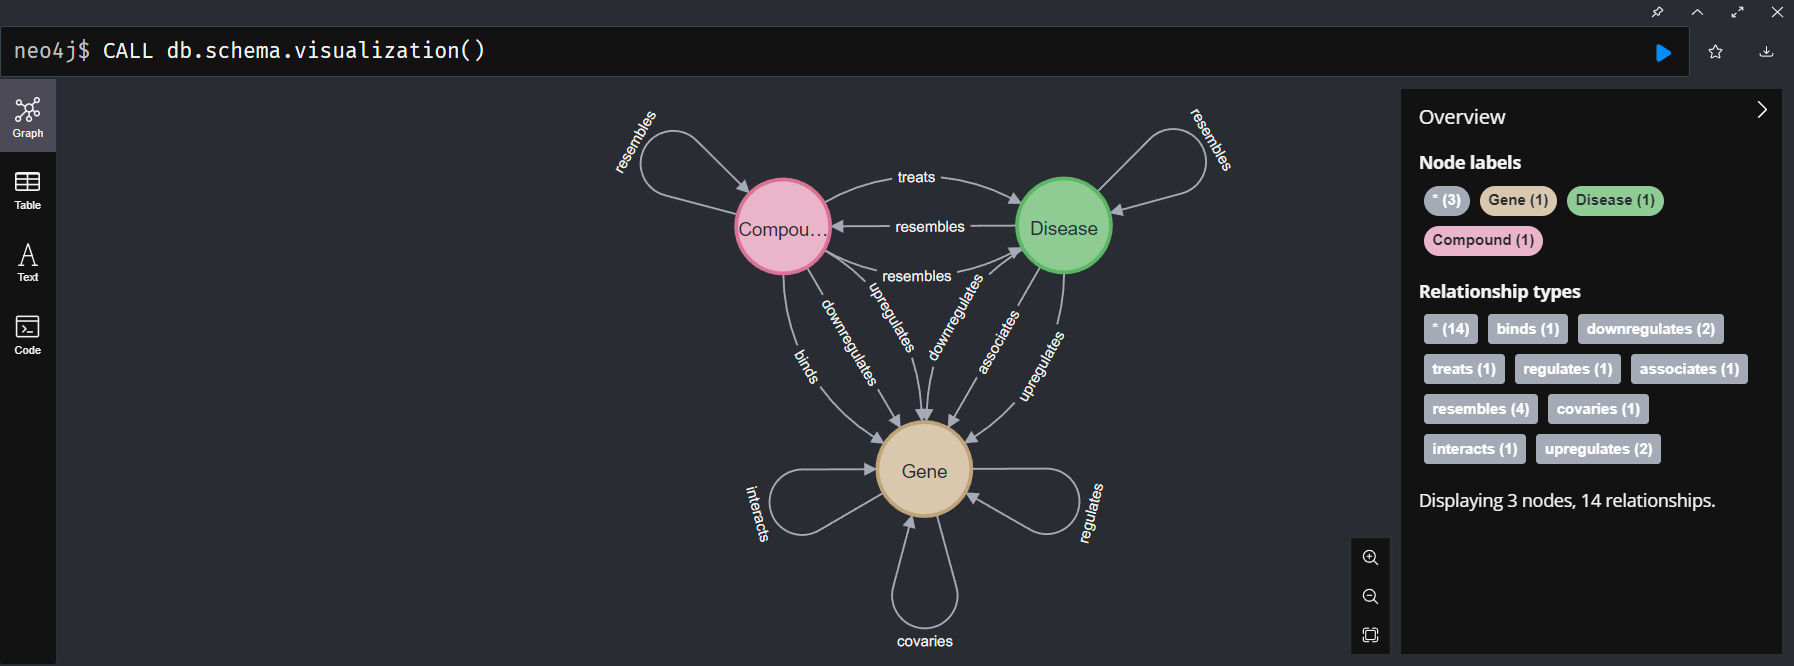
\includegraphics[width=\textwidth]{images/neo4j-setup/7}
        \caption{Visualizing schema.}
    \end{subfigure}

    \caption{Steps for Neo4j Desktop Setup.}
    \label{fig:neo4j-setup}
\end{figure}

Upon successful import, the schema can be visualized using the following Neo4j query: \texttt{CALL db.schema.visualization()}.
The resulting graph, illustrates key entities and relationships that form the basis for multi-class link prediction and knowledge graph completion in subsequent tasks.

\subsection*{Model Evaluation}
\label{model-evaluation}
We evaluated the performance of knowledge graph completion models, with a particular focus on comparing traditional embedding models with LLM-based embeddings.
As our primary baseline, we used the RotatE model, configured with 128-dimensional embeddings and trained for 100 epochs with early stopping.
While we explored several additional models, their performance was found to be subpar, and as such, we will not discuss them further.

For evaluating the performance of the LLM-based approaches, we selected the Llama 3.2-3B model.
This model was chosen primarily for its competitive output quality while maintaining relatively low VRAM requirements.

Based on the RotatE approach, we used a new architecture which combines 128 dimensions of conventional trainable embedding with 32 dimensions of projected LLM embeddings,
created by a trainable linear layer which reduces the 3200 dimensional immutable LLM embedding.

For creating the embeddings, we used two types of inputs.
The first variant, referred to as RLM, uses only the Llama embeddings generated from the label names.
The second variant incorporates Wikidata's retrieval-augmented generation (RAG) technique, which we term RLM-A (RLM Augmented).
These inputs are then tokenized in batches of 32, with a maximum sequence length of 128 tokens.
These tokenized inputs are then passed through the Llama model, and the embeddings are derived from the final hidden layer.
Specifically, the first token's hidden state (similar to a [CLS] token) is selected to represent the input, resulting in a fixed-size vector for each label.
These embeddings are stored in a pre-allocated tensor on the same device as the model, ensuring computational efficiency during processing.

This approach leverages both the strengths of RotatE in learning relational embeddings and the capacity of Llama embeddings for representing complex label information,
enhanced by additional knowledge from Wikidata entries in the RLM-A variant.
